\section{Handlers and algebraic effects}\label{sec:handlers-and-effects}
Algebraic effects and handlers have their foundation in category theory \cite{Plotkin2001a,Plotkin2013}. Plotkin and Power \cite{Plotkin2001b,Plotkin2001a} gave a categorical treatment of algebraic effects. The term ``algebraic'' implies that an effect ought to be accompanied by a set of equations, however we will only consider free algebras, which implies the theories we consider are equationless. Therefore we will not delve into the theoretical foundations of algebraic effects and handlers, rather, we will take a more pragmatic approach. Moreover, we will use the terms algebraic effect and effect interchangeably.

\subsection{Algebraic effects}
An algebraic effect is a collection of operation signatures \cite{Lindley2014}. For example, we might define an algebraic effect \type{Choice} for making a boolean choice with the following signature:
\[ \type{Choice} \defas \{ \type{Choose}: () \to \type{Bool} \} \]
Here \type{Choose} is a nullary operation whose return type is boolean. The effect \type{Choice} is the singleton set whose only member is \type{Choose}. 

The operation \type{Choose} is abstract, that is, it has no concrete implementation. We say that computations composed from algebraic effects are \emph{abstract computations}. Without handlers abstract computations are meaningless as handlers faithfully interpret effects by instantiating them with concrete implementations. 

\subsection{Effect handlers}
Benton and Kennedy generalised exception handlers \cite{Benton2001} (as known from SML, C\#, Java, etc) to expose a continuation to the programmer. Later their work was adapted by Plotkin and Pretnar \cite{Plotkin2013} to include arbitrary effects, thus they pioneered handlers for algebraic effects.

Intuitively, an effect handler is a generalised function which takes an abstract computation as input, and interprets the operations that may be discharged during evaluation of the computation. 

\subsection{Interpreting effects as computation trees}\label{sec:effects-as-computation-trees}
%An abstract computation is a syntactic structure composed from abstract operations without a particular semantics. Handlers instantiate abstract operations to turn abstract computations into concrete computations. %In addition, evaluation of a concrete computation produces an output value. Therefore, handlers essentially ``folds'' 
To develop intuition about handlers and effects we illustrate a diagrammatic interpretation of effects as computation trees \cite{Lindley2014}. We are going to assign different semantics to the same abstract computation:
\begin{lstlisting}[style=haskell]
x = if Choose() then 2
    else 4
y = if Choose() then 8
    else 16
x + y 
\end{lstlisting}
The expression assigns either the value 2 or 4 to the variable \code{x}, and similarly, it assigns either 8 or 16 to the variable \code{y}, and adds \code{x} and \code{y}.
We can picture this expression as a tree where the nodes encode operations. The range of an operation determines the number of children. In this example the range of \code{Choose} is \type{Bool} which have two members: \code{true} and \code{false}. Therefore, \code{Choose}-nodes will have two children. Leaves encode concrete values (results, i.e. \code{x + y}). Figure \ref{fig:condexp} depicts the above expression as a computation tree.
\begin{figure}[t]
\begin{center}
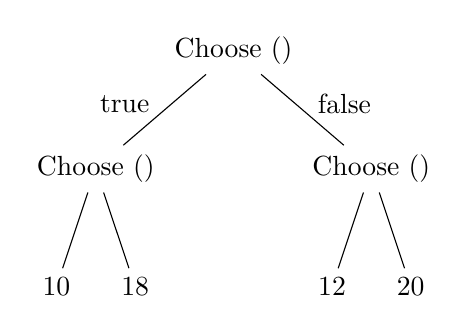
\begin{tikzpicture}[level distance=1.5cm,
level 1/.style={sibling distance=3.5cm},
level 2/.style={sibling distance=1cm}]
%\tikzstyle{every node}=[circle,draw]

\node (Root) [draw=none,rectangle] {Choose ()}
    child { node[draw=none] (q0) {Choose ()} 
      child { node[draw=none] (q00) {10}
      }
      child { node[draw=none] (q01) {18} 
      }
      edge from parent node [draw=none,left,xshift=-2.0,yshift=2.0] {true}
    }
    child { node [draw=none] (q1) {Choose ()}
      child { node[draw=none] (q10) {12}
      }
      child { node[draw=none] (q11) {20}       
      }
      edge from parent node [draw=none,right,xshift=2.0,yshift=2.0] {false}
    };
\end{tikzpicture}
\end{center}\caption{Interpretation of the conditional expression as a computation tree. The left edges correspond to \code{Choose} being instantiated with \code{true}. Analogously, the right edges correspond to an instantiation of \code{Choose} with \code{false}.}\label{fig:condexp}
\end{figure}

During evaluation of the expression we eventually have to interpret the root node \type{Choose} in Figure \ref{fig:condexp} and possibly its immediate subtrees.
There are multiple possible interpretations. One interpretation is to always interpret \type{Choose} as \code{true} which figuratively corresponds to taking the left branch. The node we arrive at is also a \type{Choose}-node, so again we choose the left branch to arrive at a leaf that contains the concrete value $10$. Hence under this interpretation the handler collapses the computation tree into the leaf $10$. Dually, we could always choose false which leads to the output value $20$. Figures \ref{fig:positive} and \ref{fig:negative} illustrate the two interpretations respectively.
\begin{figure}[b!]
    \centering
    \begin{subfigure}[t]{0.5\textwidth}
        \centering
\begin{tikzpicture}[level distance=1.5cm,
level 1/.style={sibling distance=3.5cm},
level 2/.style={sibling distance=1cm}]
%\tikzstyle{every node}=[circle,draw]

\node (Root) [draw=none,rectangle] {Choose ()}
    child { node[draw=none] (q0) {Choose ()} 
      child { node[draw=none] (q00) {10}
      }
      child { node[draw=none] (q01) {18} 
      }
      edge from parent node [draw=none,left,xshift=-2.0,yshift=2.0] {true}
    }
    child { node [draw=none] (q1) {Choose ()}
      child { node[draw=none] (q10) {12}
      }
      child { node[draw=none] (q11) {20}       
      }
      edge from parent node [draw=none,right,xshift=2.0,yshift=2.0] {false}
    };
\draw[->,black,rounded corners,dashed,line width=0.7pt]
     ($(Root) +(-1.0,0.2)$) --
     ($(q0) +(-1.0,0.4)$) --
     ($(q00) +(-0.3,0.0)$);
\end{tikzpicture}
        \caption{The ``positive'' interpretation: Always choose true. Output: 10.}\label{fig:positive}
    \end{subfigure}%
    ~ 
    \begin{subfigure}[t]{0.5\linewidth}
        \centering
 \begin{tikzpicture}[level distance=1.5cm,
level 1/.style={sibling distance=3.5cm},
level 2/.style={sibling distance=1cm}]
%\tikzstyle{every node}=[circle,draw]

\node (Root) [draw=none,rectangle] {Choose ()}
    child { node[draw=none] (q0) {Choose ()} 
      child { node[draw=none] (q00) {10}
      }
      child { node[draw=none] (q01) {18} 
      }
      edge from parent node [draw=none,left,xshift=-2.0,yshift=2.0] {true}
    }
    child { node [draw=none] (q1) {Choose ()}
      child { node[draw=none] (q10) {12}
      }
      child { node[draw=none] (q11) {20}       
      }
      edge from parent node [draw=none,right,xshift=2.0,yshift=2.0] {false}
    };
\draw[->,black,rounded corners,dashed,line width=0.7pt]
     ($(Root) +(1.0,0.2)$) --
     ($(q1) +(1.0,0.4)$) --
     ($(q10) +(1.3,0.0)$);
\end{tikzpicture}
        \caption{The ``negative'' interpretation: Always choose false. Output: 20.}\label{fig:negative}
    \end{subfigure}\caption{Two different interpretations.}    
\end{figure}
Alternatively, we could make a random choice between true and false at each branch. Again, this interpretation leads to one single output value. Albeit, the output value would be non-deterministic under this interpretation. 

Yet another interpretation is to enumerate all possible choices. For example, we can decide to explore the left branch and thereafter the right branch at each node. This interpretation corresponds to performing a depth-first traversal of the computation tree. Therefore, under this interpretation the computation tree collapses into a set of its leaves. Figure \ref{fig:enumerate} illustrates the tree traversal.
\begin{figure}[t]
\begin{center}
\begin{tikzpicture}[level distance=1.5cm,
level 1/.style={sibling distance=3.5cm},
level 2/.style={sibling distance=1cm}]
%\tikzstyle{every node}=[circle,draw]
\node (Root) [draw=none,rectangle] {Choose ()}
    child { node[draw=none] (q0) {Choose ()} 
      child { node[draw=none] (q00) {10}
      }
      child { node[draw=none] (q01) {18} 
      }
      edge from parent node [draw=none,left,xshift=-2.0,yshift=2.0] {true}
    }
    child { node [draw=none] (q1) {Choose ()}
      child { node[draw=none] (q10) {12}
      }
      child { node[draw=none] (q11) {20}       
      }
      edge from parent node [draw=none,right,xshift=2.0,yshift=2.0] {false}
    };
\draw[->,black,rounded corners,dashed,line width=0.7pt]
     ($(Root) +(-1.0,0.2)$) --
     ($(q0) +(-1.0,0.4)$) --
     ($(q00)  +(-0.5,0.0)$) --
     ($(q00)  +(-0.4,-0.35)$) --
     ($(q00)  +(0.0,-0.5)$) --
     ($(q00)  +(0.4,-0.35)$) --
     ($(q00)  +(0.5,0.0)$) --
     ($(q0)  +(-0.005,-0.3)$) --
     ($(q01)  +(-0.35,-0.35)$) --
     ($(q01)  +(0.0,-0.45)$) --
     ($(q01)  +(0.35,-0.35)$) --
     ($(q01)  +(0.4,0.0)$) --
     ($(q0)   +(1.0,0.5)$) --
     ($(Root) +(-0.3,-0.4)$) --
     ($(q1)  +(-0.8,-0.1)$) --
     ($(q10)  +(-0.5,0.0)$) --
     ($(q10)  +(-0.4,-0.35)$) --
     ($(q10)  +(0.0,-0.5)$) --
     ($(q10)  +(0.4,-0.35)$) --
     ($(q10)  +(0.5,0.0)$) --
     ($(q1)  +(-0.005,-0.3)$) --
     ($(q11)  +(-0.35,-0.35)$) --
     ($(q11)  +(0.0,-0.45)$) --
     ($(q11)  +(0.35,-0.35)$) --
     ($(q11)  +(0.4,0.0)$);
\end{tikzpicture}\caption{Enumerate all possible choices. Output: $\{10,18,12,20\}$.}\label{fig:enumerate}
\end{center}
\end{figure}

Essentially, our interpretations (handlers) correspond to particular folds over syntax trees (abstract computations) \cite{Kammar2013}.